\documentclass[11pt,twoside]{report}
\usepackage{preamble}
\graphicspath{{../img/ch4/}}
\setcounter{chapter}{3}


\begin{document}

\chapter{Tracking fish in 3D}

\epigraph{Something clever.}{Someone important}

This chapter would present the method to build up a 3D tracking system for the zebrafish, and the results obtained from the custom 3D tracking system. This tracking system is inspired by the pioneering work of \citeauthor{cavagna2008} \cite{cavagna2008} and \citeauthor{kelley2013} \cite{kelley2013}, where the 3D trajectories of European starlings and midges were calculated. Performing the same task on the fish schools is a tougher job for the refraction on the water--air interface, and the way to handle the refraction would be discussed.

To carry out the 3D tracking, it is important to understand the formation of the image on a camera, because one needs to reverse the formation process to get the 3D locations. The formation of images on a camera is identical to the way we perceive the world visually, and it will be covered as a brief introduction of projective geometry in this chapter. With the mathematical basis of projective transformations, I will introduce the pinhole camera model, including the practical ways to calibrate the cameras. The knowledge of the projective geometry and camera model would enable one to find 3D locations of objects from different 2D images.

However, the real measurements are never perfect. The 2D measurements of the fish positions can be problematic, as described in the previous chapter. In addition, new errors would also emerge from the camera calibration process, as well as the wrong association of identities in different views (different cameras). The errors create ambiguities during the locating of 3D coordinates, and some practical ways to cope with the ambiguities would be discussed in this chapter. To validate the developed methods, I will track a simulated fish data, and assess the accuracy of the 3D tracking method.

Applying the tracking method, I will present the 3D behaviours of wildtype zebrafish with different group sizes. Some descriptive quantities such as density distribution, average speed, and degree of polarisation would also be presented. Inspired by the soft--matter community, I also calculated some correlation functions to characterise the spatial and temporal features of the system. These quantities and correlation functions will serve as the final target for modelling the zebrafish in the next chapter.

\section{Three Dimensional Computer Vision}

\subsection{The Projective Geometry}

This subsection include a very brief introduction to the homogeneous coordinates, projective space, and the hierarchy of projective transformations. Hopefully it will provide the readers the mathematical basis, which would be very helpful for implementing the algorithms introduced later in this chapter. More details on this subject is available in the celebrated text book by \citeauthor{hartley2003} \cite{hartley2003}.
 
 
I will begin the introduction with the definition of homogeneous coordinates, where a normal Euclidian coordinate, say $(x, y)$ in $\mathbb{R}^2$, is uniquely represented as $(x, y, 1)$, which satisfies the following property
 
 $$
 (x, y, 1) = (kx, ky, k).
 $$
 
 \noindent This new vector with an extra ``1'' is called the homogeneous vector. The mapping from the Euclidian coordinates to their homogeneous counterparts is one-to-one and onto, and the \emph{inhomogeneous} representation of homogeneous vector $(x_1, x_2, x_3)$ is $(x_1/x_3, x_2/x_3)$. The projective transformation (to be introduced later) can be easily expressed as matrix multiplication of a $3 \times 3$ matrix and a $3 \times 1$ homogeneous vector, and this is the reason people slid an extra number into the homogeneous coordinates (represented by a homogeneous vector). The space 
 
The next concept to be introduced is the projection transformation. One daily example of projection is the formation of shadows. Figure \ref{fig:projection-seagull} shows the shapes of a seagull and its shadow in a photo. Looking at these shapes separately, it is obvious that there are certain distortion involved. The transformations between these shapes are projection transformations.


\begin{SCfigure}
	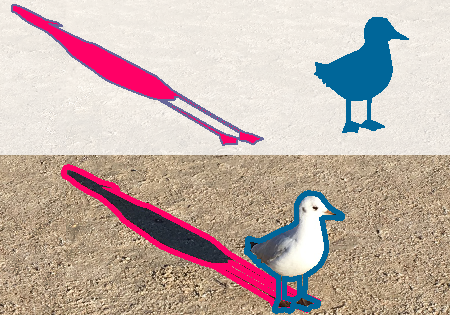
\includegraphics[width=0.6\linewidth,outer]{projection-seagull}
	\caption{The photo of a seagull and its shadow on the beach, taken by the author. The shape of the seagull and its shadow is outlined, and these two geometric shapes were separated on the top, stressing the distortion.}
	\label{fig:projection-seagull}
\end{SCfigure}

 
% The affine transformation is commonly seen in ancient Chinese paintings. One example is illustrated in Fig.\ \ref{fig:affinity_example}. The shape of tables, the rectangles, were drawn as parallelograms, as the result of affine transformation. The key feature of such transformation is the fact that it kept the parallelisation of lines. Figure \ref{fig:affinity_example} seems a bit unnatural, because we perceive the world after \emph{projective} transformation instead of the affine transformation. The projective transformation could be expressed as.
%
% 
%  \begin{SCfigure}
%  \includegraphics[width=0.6\linewidth,outer]{affinity-example}
%  \caption{The affinity transformation in the ancient art of Tang dynasty. The shapes of the tables were highlighted, and they were the results of affine transformation of a rectangle. The painting described a typical situation of a party among the elite class of its time. The author of the work can not be identified, and it is now kept in the national palace museum, Taiwan (K2A000815N000000000PAA).}
%  \label{fig:affinity_example}
%\end{SCfigure}
%
% 
% The Western artists applied the projective transformation in their works widely during the \emph{Rinascimento} and afterwards, yielding visually realistic paintings. One famous example is the \emph{The School of Athens} in the apostolic palace in Vatican, illustrated in Fig.\ \ref{fig:projective_example}. As a result of the projective transformation, the originally parallel lines would not be parallel with each other. However, the collinearity is invariant w.r.t. such transformation. This means a line would still be a line, instead of a being a curve.
% 
% 
% 
%\begin{SCfigure}
%	\centering
%	\includegraphics[width=0.6\linewidth,outer]{projective-example}
%	\caption{The projective transformation in \emph{The School of Athens} by Raphael. The shapes of the floor tiles were highlighted, and they were the results of projective transformation of a rectangle. The painting exhibited a group of intellectually advanced human beings.}
%	\label{fig:projective_example}
%\end{SCfigure}



\subsection{Modelling the Camera}


In order to analyse the images taken by the camera, it is necessary to understand the projective transformations involved in the formation during the process of photography. The cameras that we use everyday can be effectively described by the pin--hole camera model, which is illustrated in Fig. \ref{fig:camera_model}.

\begin{SCfigure}
  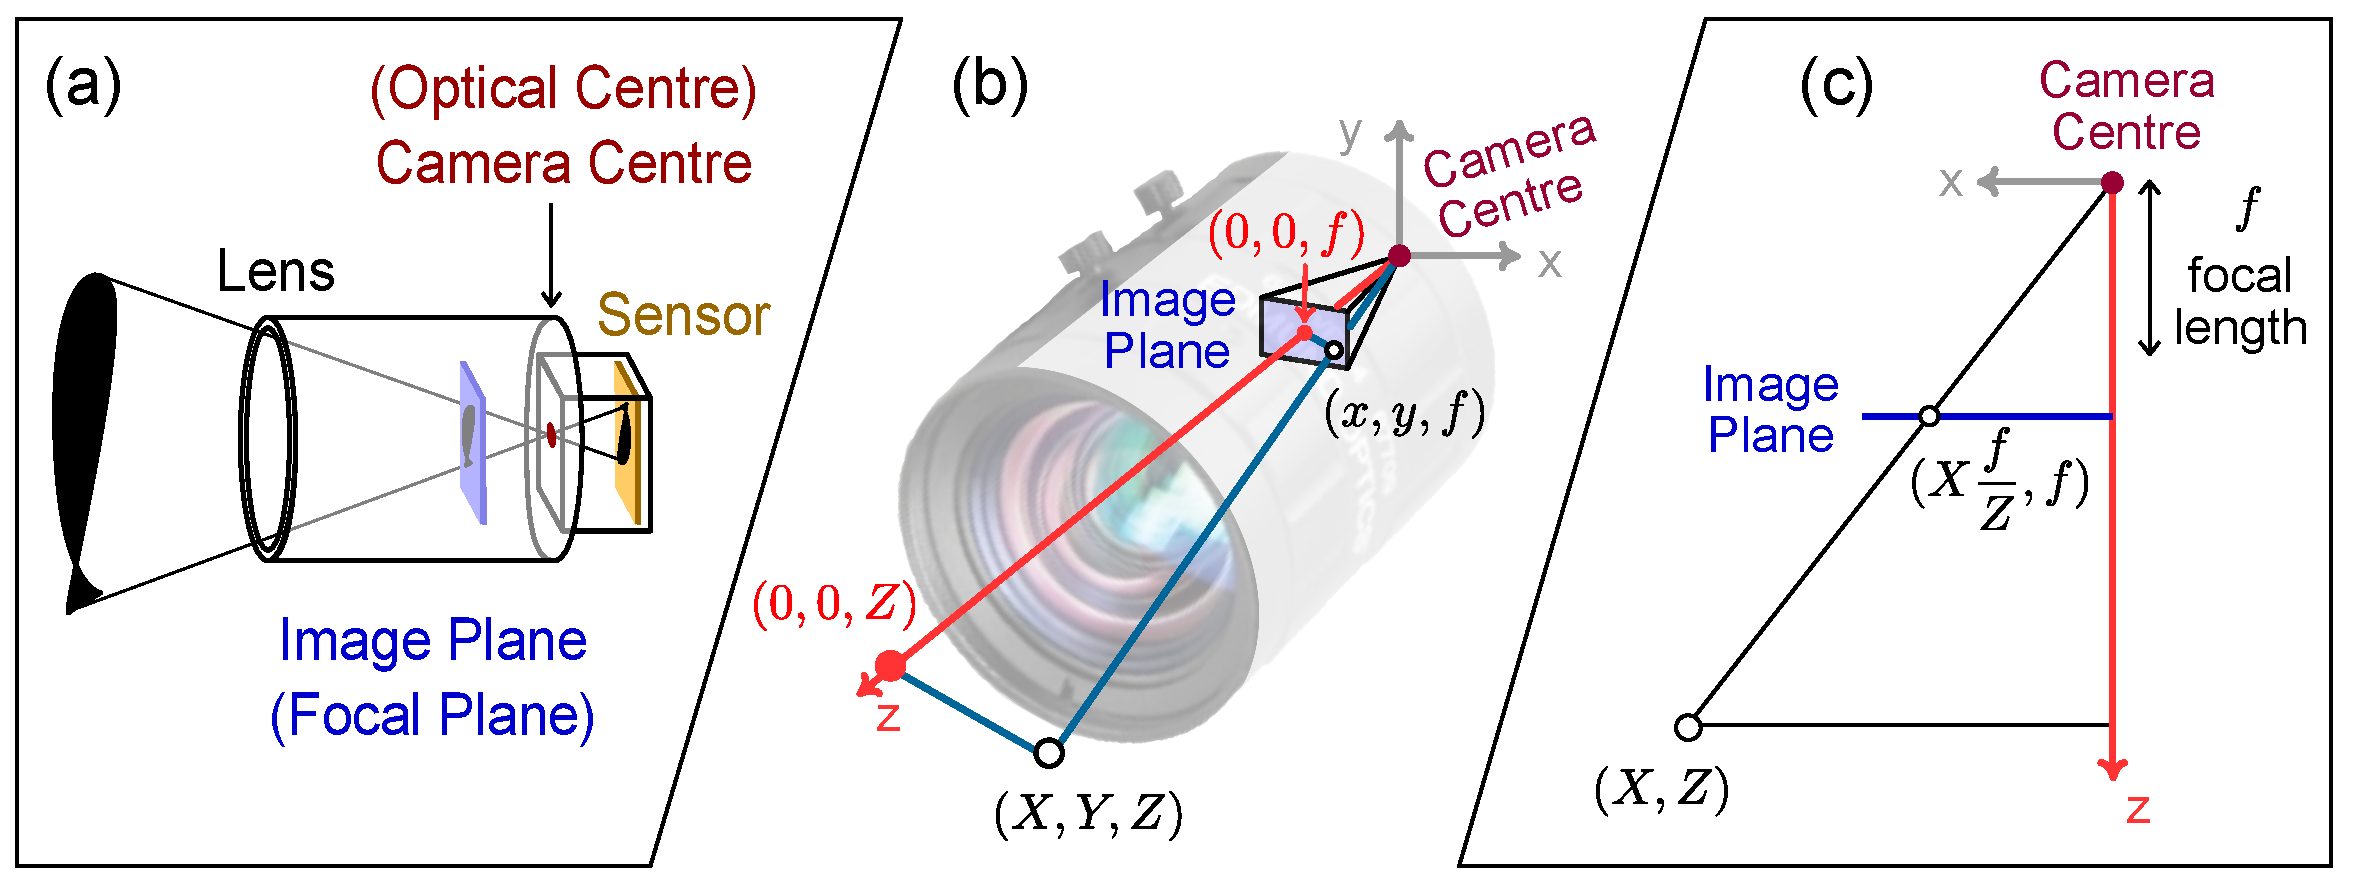
\includegraphics[width=0.6\linewidth,outer]{camera-model}
  \caption{The pinhole camera model and the coordination system of the camera. The top figure shows the general ideal of the pinhole model, where the object in the real world projected its inverted image onto the sensor of the camera. Equivalently, one might think of this process as forming a projected, but not inverted image, onto a virtual image plane. The bottom figure shows the coordination system centred at the focal point, often referred to as the ``camera basis''. The point $(X, Y, Z)$ would be projected onto the image plane, with coordinates $(x, y, 1)$.}
  \label{fig:camera_model}
\end{SCfigure}

\subsubsection{Calibrating Cameras}

\subsubsection{Manual Calibration with Conic Homographies}

The calibration method using the chessboard is convenient and easy. However, there is an excess of information in such method, and one can perform the camera calibration with just the geometry of the fish tank. In this sub section, I will exploit the fact that the radial symmetry fish tank to calculate the extrinsic parameters of the cameras.

\begin{SCfigure}
  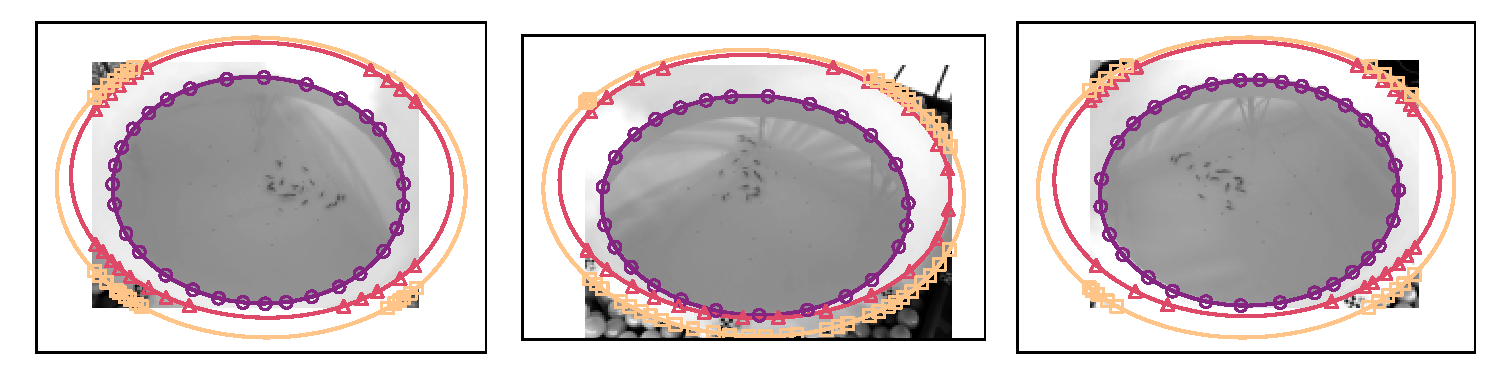
\includegraphics[width=1\linewidth,outer]{conics-measure}
  \caption{The conic features measured from the undistorted image. These feature points were fitted to get the conic matrices ($\mathbf{C}_{j}^{i}$ for the $j$th circle in camera $i$).}
  \label{fig:conic_measure}
\end{SCfigure}


This manual calibration is more tedious than the automated version. However, it can serve as an alternative way to assess the quality of the chessboard calibration method. The conic feature calibration method could also be applied if the cameras were moving/rotating, to capture larger animal groups.


\section{Building the Tracking System}

This section should serve as a practical tutorial for building a multiple view 3D system to track animals. The current system is capable of extracting 3D trajectories with commercial cameras and lenses, but it is not the only solution for such task. Instead, there are alternative ways to follow the movement of animals such as binding animals with global positioning system (GPS) \cite{nagy2010} and tagging the animal bodies \cite{jolles2017}.

\subsection{Tank Design and the Hardwares}

Figure \ref{fig:lab} shows the experimental setup in the laboratory, where I mounted 3 cameras pointing to a bowl--shaped tank. This big bowl was immersed in a framed swimming pool, and the swimming pool was covered with plastic balls\marginfootnote{Curiously, immersing plastic balls inside the fish tank is also something physicists do to explore the structure of the simple liquid in 1930s. \cite{travis2021}} to reduce the evaporation of water. Synchronised signals were generated with a Arduino chip, and the cameras are able to capture time--synchronised videos with the signals. The trigger signal for the camera is a 5V pulse, being the default \texttt{HIGH} output signal of an Arduino chip.


The big, white plastic bowl was specially designed and manufactured to contain the fish. The choice of the shape was based on the fact that the fish tend to stay in the corner of the tank, when they entered an unfamiliar environment. Using a bowl--shaped container prevented the aggregation at the corners. Except for the corner effect, the bowl also provides no blind zone for all of the cameras, preventing the systematic disappear and reappearing of the fish in the video.


The zebrafish are living animals, and it is also important to provide them a suitable condition. Typically, the fish need a temperature between 25 \degree C and 30 \degree C, and the water should be constantly filtered and sterilisation with UV light. All of the related equipments re placed outside the bowl--shaped tank, but inside the swimming pool, so that they would not affect the behaviours of the fish.


\begin{SCfigure}
  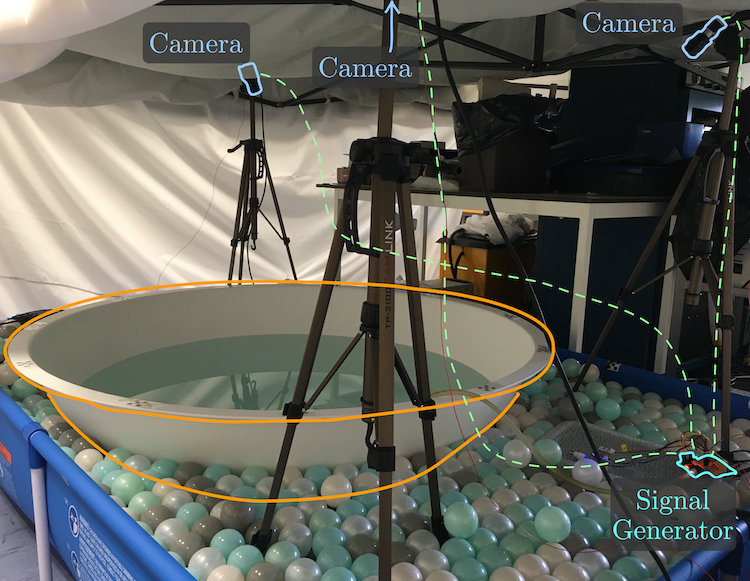
\includegraphics[width=0.8\linewidth,outer]{lab.jpg}
  \caption{The photo of one experimental setup. Three cameras were mounted to observe the fish in the bowl shaped tank. Time--synchronised signals were generated by a Arduino chip to trigger the cameras for capturing synchronised videos. The bowl was immersed in a bigger tank, which is a framed swimming pool. The husbandry--related equipments, such as the water filter, the heaters, the UV lamp, were placed outside the bowl but inside the bigger tank.}
  \label{fig:lab}
\end{SCfigure}


I also measured the 3D shape of the tank to know the exact boundary for the fish. The measurement was performed by placing markers on the surface of the tank, and then reconstruct the markers in 3D. Since the tank is rotationally symmetric around the z--axis, it is appropriate to describe its geometry in the cylindrical coordination system with the hight ($Z$) and the radius ($R$). Figure \ref{fig:tank} shows the results of the measurement, and the shape of the tank can be modelled by function $Z=0.734 R^2$, where both length variables take the units of millimeter. The shape of the tank, together with the water level, are the boundaries for the movement of the fish.

\begin{SCfigure}
  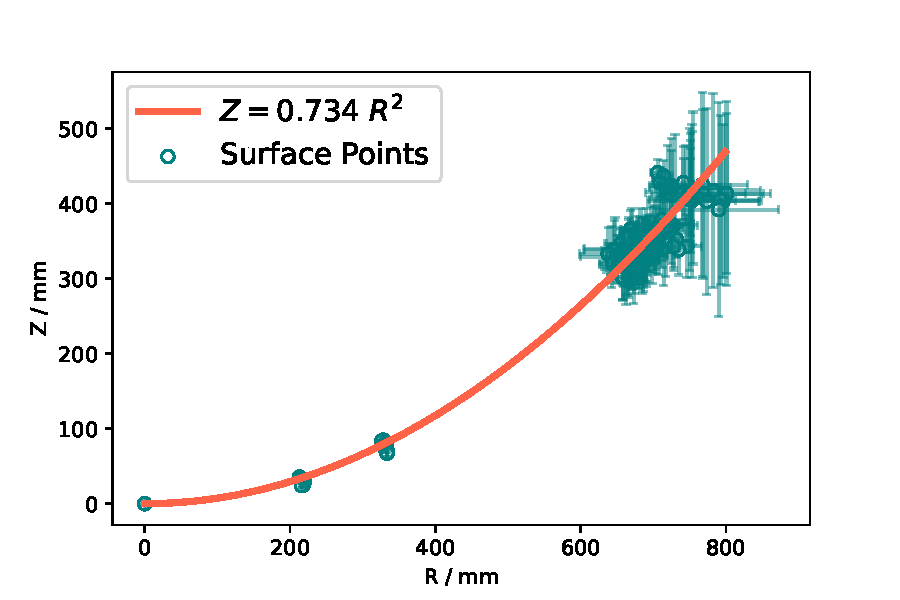
\includegraphics[width=0.8\linewidth]{tank-fit.pdf}
  \caption{The measured shape of the observation tank. The scatters were markers on the tank, which were fitted by function $Z=0.734R^2$, where the unit of both $Z$ and $R$ is millimetre.}
  \label{fig:tank}
\end{SCfigure}


\subsection{Handling the Refraction}



\subsection{Locating Fish in 3D}

The task of finding the 3D positions of zebrafish consists of two parts. The first part is finding the positions of fish in individual views, and the method is discussed in the previous chapter. The second part is to integrating the positions from different views and the knowledge of about the cameras, to calculate the 3D locations.


\begin{SCfigure}
  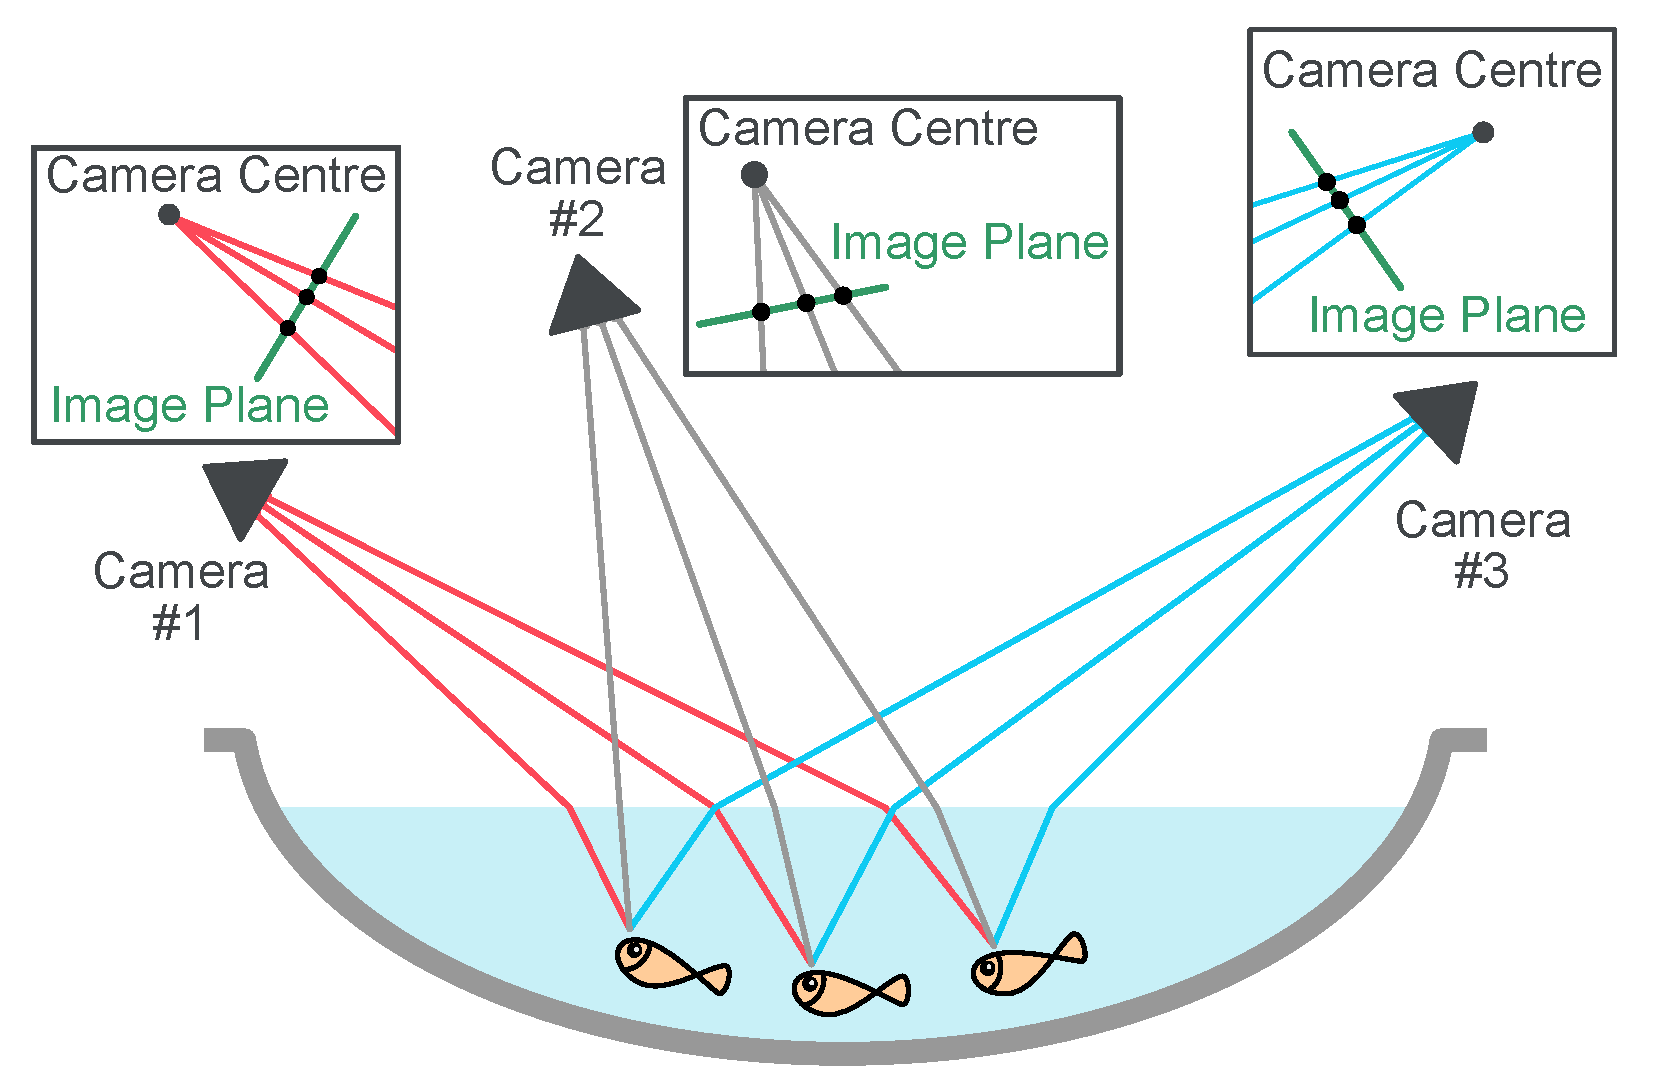
\includegraphics[width=0.8\linewidth]{track-3d-idea}
  \caption{Tracking the fish with three cameras. This figure demonstrates the idea of obtaining the 2D locations of fish with the input of 1D information. Each inserted box shows the projection of the fish onto the camera. Knowing the location of the centres (the focal points) of the cameras, one can re-cast the rays responsible for the projection of the fish. The intersections of the re-casted rays are the locations of the fish.}
  \label{fig:track_idea_3d}
\end{SCfigure}

\pagebreak

\subsection{Framework Design}

To the best of my knowledge, there is no framework nor libraries\marginfootnote{The term ``library'' refers to a collection of reusable code, which can be called by the user. The term ``framework'' refers to a collection of libraries and other utilities, which functions with the input of the user. The example of a library is ``Numpy'', which provides efficient n--dimensional array operations. The example of a framework is the Large-scale Atomic/Molecular Massively Parallel Simulator (LAMMPS), which read the user input file and perform molecular dynamic simulations.}
for the reconstruction of 3D trajectories from synchronised multiple--view videos at the time of this research (from 2018 to 2022). Therefore, I have to write all the analysing code from scratch, which turned out to be a real challenge in terms of software engineering. Developing the software is difficult because the 3D reconstruction process are composed of many small tasks, for instance the 2D feature selection and the camera calibration. New features and algorithms were frequently added to cope with different tasks, which would inevitably increase the complexity of the framework/library. If not being careful with the complexity, the code may eventually end up being not maintainable, forbidding its further improvement.

The way I organised my framework is summarised by the tree below. Each node represent either a directory (with capitalised first letter) or a file (with lower case letters). For instance, \code{Executable} is a folder and \code{exec_task_1} is a file.

\begin{diagram}
	\dirtree{%
	.1 Framework.
	.2 Executable\marginfootnote{\textrm{It is convenient to add the \texttt{Executable} directory to the \texttt{PATH} environment variable, so that we can call these executable files directly.}} (Called by the user).
	.3 exec\_task\_1.
	.3 exec\_task\_2.
	.2 Script (Calls the library).
	.3 Task\_1.
	.4 scirpt.py.
	.4 config.ini (user input provided by the executable).
	.3 Task\_2.
	.4 ....
	.2 Library\marginfootnote{\textrm{I used Python as the main script language. In my case, it is very convenient to add the \texttt{Library} directory to the \texttt{PYTHONPATH} environment variable, so that one can directly import the modules.}}.
	.3 Module\_1.
	.4 foobar.py.
	.4 hoge.so.
	.4 tutu.a.
	.3 Module\_2.
	.4 ....
}
\end{diagram}

The users interact with the framework only through the executables. The user is expected to run the executable from a working directory (\code{PWD}). The executables would copy a task folder (\code{Framework/Script/Task_1}) to \code{PWD/Task_1}. The user input would handled by changing the configuration file (\code{config.ini}), and the results would be obtained by executing the script (\code{script.py}). The generated result will be kept inside the copied task folder (\code{PWD/Task_1}). The task folders can be ``volatile'', and suffer from frequent changes and errors. This volatility is acceptable, since each task is a self--contained unit, as the script and configuration file uniquely determines the obtained result.

All of the implemented algorithms (subroutines, functions, classes) were placed inside the library (\code{Framework/Library}), and they are called by the scripts. These algorithms need much more attention than the scripts, and they ideally require careful tests. If a function in the algorithm provides a wrong answer, then all the scripts calling this function needed to be re-calculated, affecting potentially many tasks. In addition, the different modules should not depend on each other\marginfootnote{In terms of Python, it means the \texttt{*.py} files in \texttt{Module\_1} would not import from other modules, and vice versa.}, in order to reduce the complexity of the library.

With such structure, it is easy and clear to add new functions for new tasks. For instance, if I want to perform a new task (\code{T}) with a new algorithms (\code{A}), I will create the collection of script, for task \code{T}, under the folder \code{Framework/Script}. Also, I would implement algorithm \code{A} inside a module, then write an executable file for the user. The following tree diagram represented the updated framework.

\begin{diagram}
	\dirtree{%
	.1 Framework.
	.2 Executable (Called by the user).
	.3 exec\_task\_1.
	.3 exec\_task\_2.
	.3 \color{teal}{exec\_T}.
	.2 Script (Calls the library).
	.3 Task\_1.
	.4 ....
	.3 Task\_2.
	.4 ....
	.3 \color{teal}{New\_Task\_T}.
	.4 ....
	.2 Library.
	.3 Module\_1.
	.4 foobar.py \color{teal}{(+ code for algorithm A)}.
	.4 hoge.so.
	.4 tutu.a.
	.3 Module\_2.
	.4 ....
}
\end{diagram}

\noindent With this clear framework structure and version control softwares (\code{git} and GitHub), I managed to maintain the fish tracking code through out the 4--year project, working seamlessly on both my personal laptop and HPC clusters.

\subsection{The Accuracy of the Method}

I evaluated the accuracy of the tracking method with the simulated data. Typically, I generated the trajectories of 50 simulated fish inside a container. Then I use the software \emph{Blender} (version 2.91.0 on Ubuntu 20.04) to render the movement of the fish as animations, with multiple cameras. The result movies looks very similar to my experimental videos, in terms of the local fish density and the speed. This similarity ensured the accuracy that I assessed from the simulation movie is valid for my experimental data.


\section{The Behaviours of Zebrafish in 3D}

\subsection{A Single Fish}

Figure



\subsection{A Pair of Fish}

\subsection{Many Fish}

\section{Conclusion}

\printbibliography

\end{document}
